\section{Projeto}

\begin{frame}
  \frametitle{Poluição do Ar em Acra, capital de Gana}
  Projeto Internacional: \\
  \textit{Poluição do Ar em Acra: Padrões temporais e espaciais e seus impactos sociais e econômicos.} \\ 
  coordenado pelo Prof. Dr. Majid Ezzati da \textit{Harvard School of Public Health}.
\end{frame}

\begin{frame}
 \frametitle{ África Subsariana (SSA)}
  As cidades da SSA tem as seguintes características: 
  \begin{itemize}
    \item População predominantemente rural;
    \item Vias não pavimentadas;
    \item Maior taxa de crescimento populacional urbano do mundo;
    \item Não possuem monitoramento de poluição do ar;
    \item Queima de biomassa para o cozimento de alimentos.
  \end{itemize}
\end{frame}

\begin{frame}
  \frametitle{Nima}
  Fotos do bairro de Nima
  \begin{figure}[H]
    \centering
    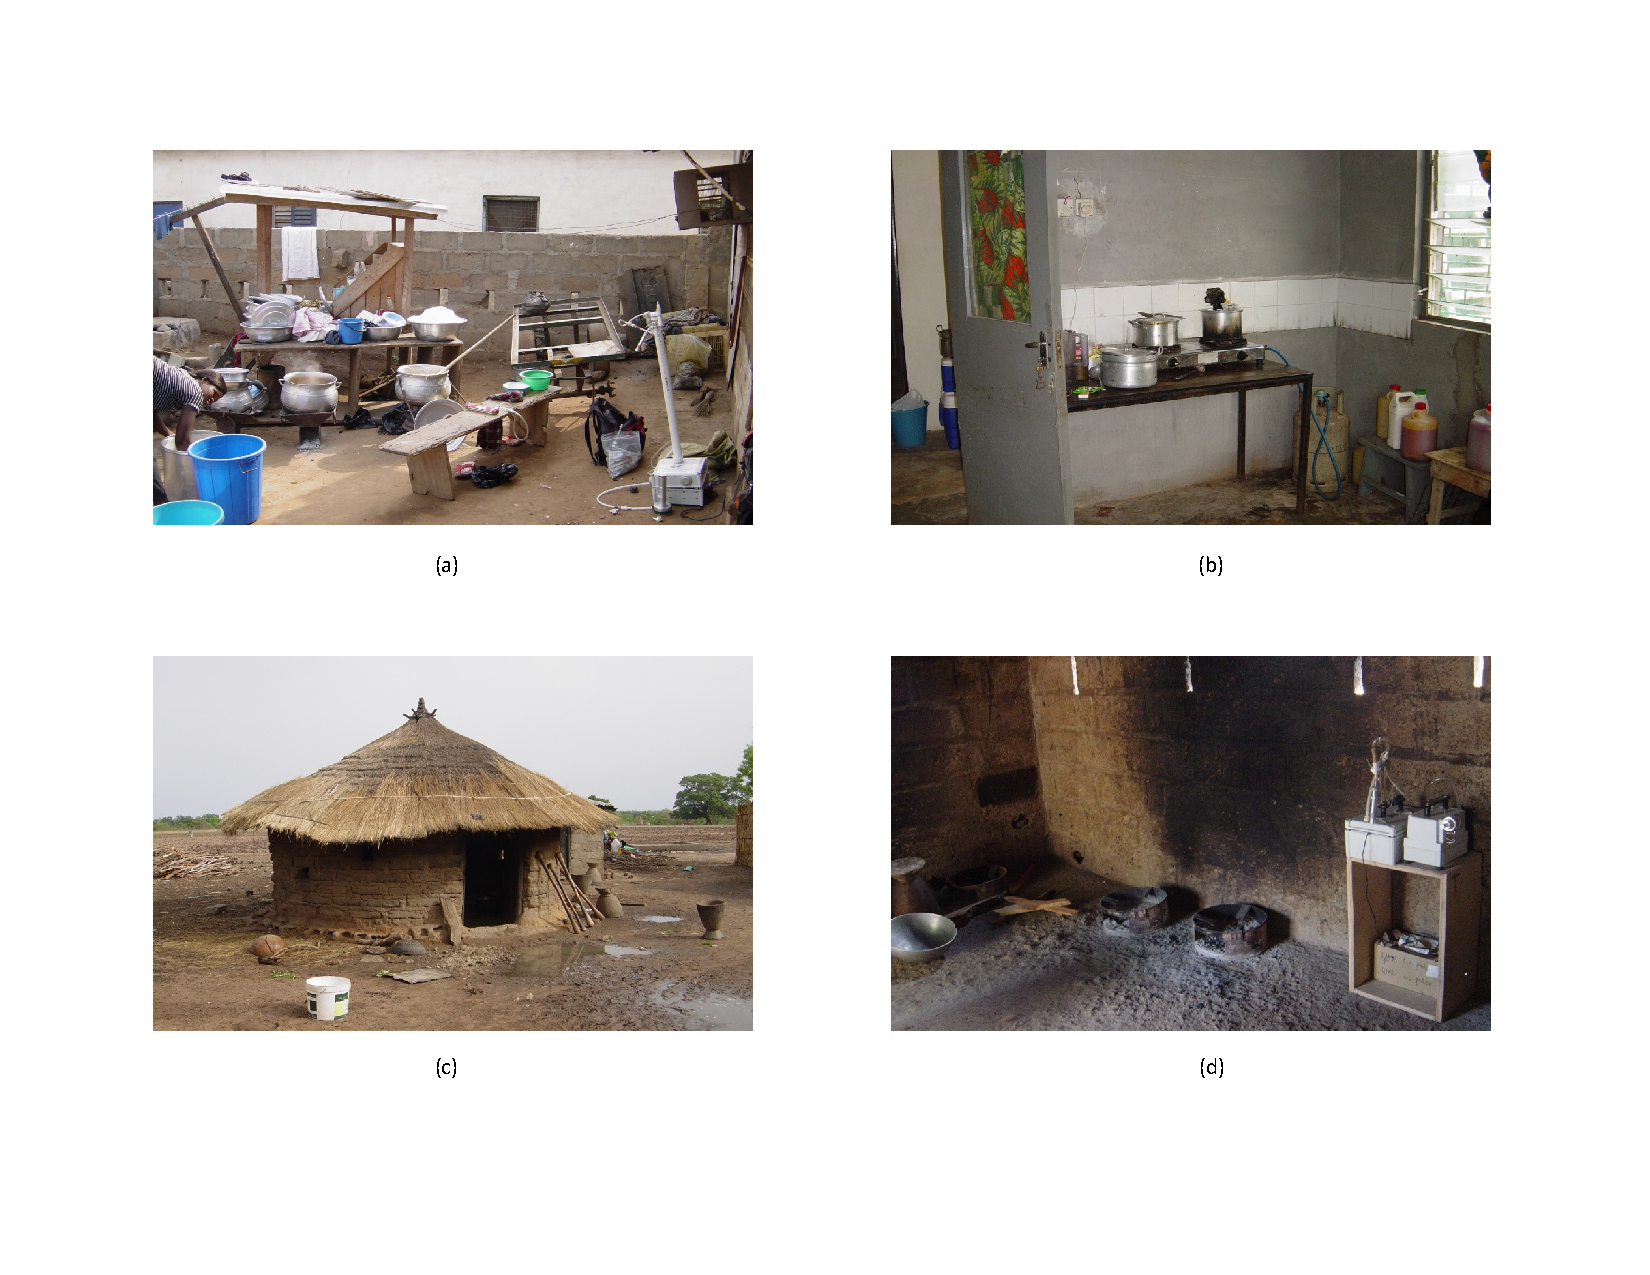
\includegraphics[scale=0.3]{../../../inputs/images/zheng/nima.pdf}
  \end{figure}
\end{frame}

\begin{frame}
  \frametitle{Gana}
  \begin{figure}[H]
    \centering
    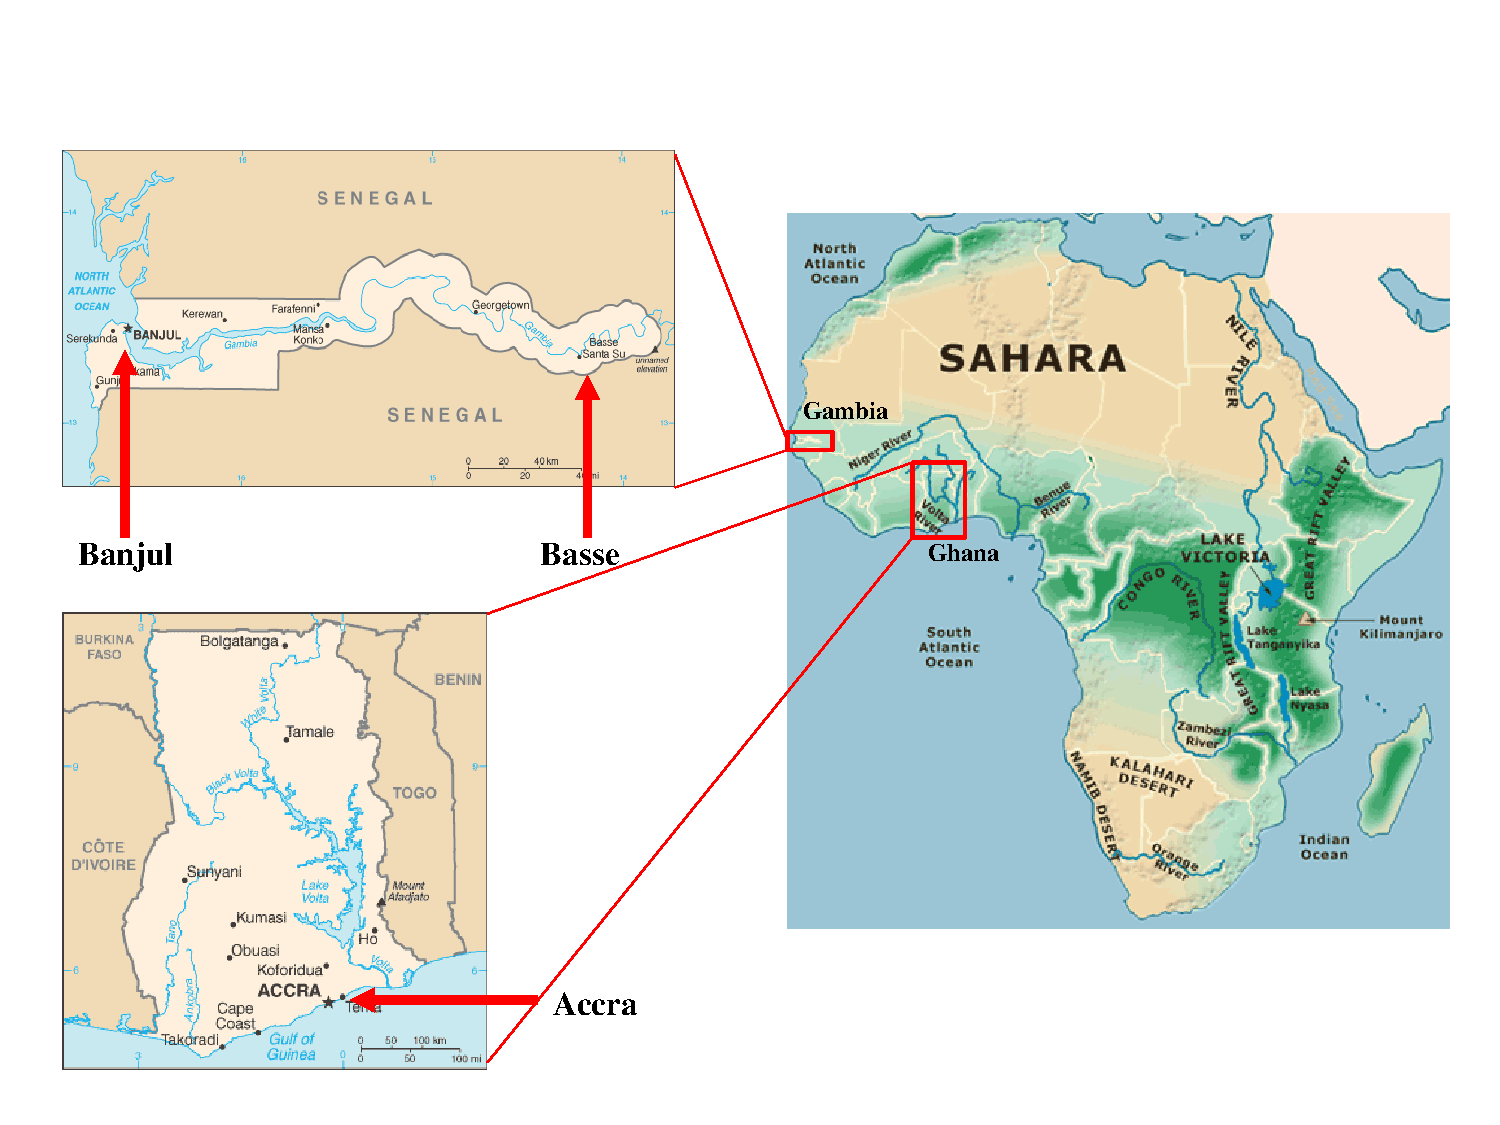
\includegraphics[scale=0.3]{../../../inputs/images/zheng/africa_ghana.pdf}
  \end{figure}
\end{frame}

